\documentclass[nooutcomes]{ximera}
\usepackage{fullpage}
%% handout
%% space
%% newpage
%% numbers
%% nooutcomes

\newcommand{\RR}{\mathbb R}
\renewcommand{\d}{\,d}
\newcommand{\dd}[2][]{\frac{d #1}{d #2}}
\renewcommand{\l}{\ell}
\newcommand{\ddx}{\frac{d}{dx}}
\newcommand{\dfn}{\textbf}
\newcommand{\eval}[1]{\bigg[ #1 \bigg]}

\renewenvironment{freeResponse}{
\ifhandout\setbox0\vbox\bgroup\else
\begin{trivlist}\item[\hskip \labelsep\bfseries Solution:\hspace{2ex}]
\fi}
{\ifhandout\egroup\else
\end{trivlist}
\fi}

\title{4.3: Graphing Functions}

\begin{document}
\begin{abstract}
\end{abstract}
\maketitle

%problem1
\begin{problem}
  \outcome{Determine how the graph of a function looks based on an analytic description of the function.}
  \mbox{}
  \begin{enumerate}
    \item
      You are given that $f''(x) > 0$ for all $x$.
      Which of the following must be true about $f(x)$ on the region $0 \leq x \leq 2$?
      \begin{enumerate}
        \item
          There is a critical point between $0$ and $2$.

        \item
          An absolute maximum occurs at either $x=0$ or $x=2$.

        \item
          There is a local maximum, but not enough information is given to determine where.

        \item
          $f$ need not have a local maximum.
      \end{enumerate}
      \begin{freeResponse}
        Only (ii) and (iv) must be true.
        The following picture provides a counterexample for both (i) and (iii):
        \begin{image}
          \includegraphics[trim= 70 470 250 190]{Figure1.pdf}
        \end{image}
      \end{freeResponse}
		
     \item
       You are told that $f''(x) > 0$ for all $x$.
       Which of the following must be true about the graph of $y=f(x)$?
       \begin{enumerate}
         \item
           The graph is a straight line.

         \item 
           The graph crosses the $x$-axis at most once.
         
         \item
           The graph is concave down.

         \item
           The graph crosses the $y$-axis more than once.

         \item
           The graph is concave up.
       \end{enumerate}
       \begin{freeResponse}
         Only (v) must be true.
         For (i), the function $f(x) = e^x$ provides a counterexample:
         \begin{image}
           \includegraphics[trim= 70 470 250 190]{Figure2.pdf}
         \end{image}
			
         For part (ii), the function $f(x) = x^2 -2$ provides a counterexample:
         \begin{image}
           \includegraphics[trim= 70 470 250 190]{Figure3.pdf}
         \end{image}
			
         Part (iii) is clearly false since $f''(x) > 0$ means that $f$ is concave up.
         Part (iv) is false for any function.
       \end{freeResponse}
    \end{enumerate}
\end{problem}


%problem2
\begin{problem}

  Sketch the graph of a function $f$ satisfying all of the conditions:
  \begin{enumerate}
    \item
      $f$ is continuous and \emph{odd}, $f(0) = 0$,

    \item
      $\displaystyle \lim_{x \to \infty} f(x) = -5$,

    \item
      $f'(x) > 0$ on $(6, \infty)$,

    \item
      $f'(x) < 0$ on $(0, 6)$,

    \item
      $f''(x) > 0$ on $(0, 12)$, and
      
    \item
      $f''(x) < 0$ on $(12, \infty)$.
  \end{enumerate}

    \begin{image}
      \includegraphics[scale = 0.07]{BlankGrid.pdf}
    \end{image}

  \begin{freeResponse} \hfil
    \begin{image}
      \includegraphics[scale = 0.049]{Graphfunction1.pdf}
    \end{image}
    \begin{image}
      \includegraphics[scale = 0.049]{Graphfunction2.pdf}
    \end{image}

    \begin{image}
      \includegraphics[scale = 0.35]{Graphfunction4.png}
    \end{image}

    \begin{image}
      \includegraphics[scale = 0.27]{Graphfunction5.png}
    \end{image}

    \begin{image}
      \includegraphics[scale = 0.27]{Graphfunction6.png}
    \end{image}

    \begin{image}
      \includegraphics[scale = 0.35]{Graphfunction7.png}
    \end{image}
  \end{freeResponse}
\end{problem}

%problem3
\begin{problem}

  Determine the following information about the given function and then graph the function:
  \[ 
    f(x) = \frac{x^2 + x + 1}{x^2}
  \]
  
  Domain\\
  $x,y$-intercepts\\
  Symmetry\\
  Asympotes\\
  Intervals of increasing/decreasing\\
  Maxima/Minima\\
  Intervals of concavity\\
  Inflection points
  
  \begin{freeResponse}
    \mbox{}
    \begin{enumerate}
      \item  
        \dfn{Domain}  \\
        
        The function is a rational function, and so the domain of the function is all real numbers except where the denominator equals zero.
        \[
          x^2 = 0 \quad \Longrightarrow \quad x=0
        \]
	So the domain of $f$ is $(-\infty ,0)\cup (0,\infty )$.


      \item
        \dfn{$x,\, y$-intercepts}  \\
        To find any $x$-intercept(s), set $y=0$ and solve:
        \begin{align*}
          \frac{x^2 + x + 1}{x^2} = 0 &\implies x^2 + x + 1 = 0 \\
          &\implies x = \frac{-1 \pm \sqrt{1-4(1)(1)}}{2(1)}
        \end{align*}
	which has no real solutions.
        Thus, $f$ has no $x$-intercepts.
			
	Since $x=0$ is not in the domain of $f$, $f$ has no $y$-intercepts as well.
 
     \item 
       \dfn{Symmetry}  \\

       Note that $f(1) = 3$ and $f(-1) = 1$.
       So it cannot be for all values of $x$ that either $f(-x) = f(x)$ or $f(-x) = -f(x)$.
       So $f$ is neither even nor odd, and therefore $f$ has no symmetry.
			
     \item
       \dfn{Asymptotes}  \\

       \dfn{Vertical Asymptotes:}  Our only candidate is $x=0$, and so we compute the two one-sided limits:
       \[
         \lim_{x \to 0^-} \frac{x^2+x+1}{x^2} = \infty 
       \]
       \[
         \lim_{x \to 0^+} \frac{x^2+x+1}{x^2} = \infty
       \]
       Therefore, $x=0$ is the only vertical asymptote of $f$.

       \dfn{Horizontal Asymptotes:}  We compute the following limits:
       \[
         \lim_{x \to \infty} \frac{x^2+x+1}{x^2} = 1
       \]
       \[
         \lim_{x \to -\infty} \frac{x^2+x+1}{x^2} = 1
       \]
       we checked both ends and so the only horizontal asymptote of $f$ is $y=1$.
			

			
     \item
       \dfn{Increasing/Decreasing}  \\

       \begin{align*}
         f'(x) &= \frac{x^2(2x+1) - (x^2+x+1)(2x)}{x^4} \\
               &= \frac{2x^3 + x^2 - 2x^3 - 2x^2 - 2x}{x^4} \\
               &= \frac{-x^2 - 2x}{x^4} \\
               &= \frac{-x-2}{x^3}
       \end{align*}
			
       To find where $f'$ is positive and where $f'$ is negative, we need to find where $f'(x) = 0$ and where $f'(x)$ does not exist.
       Clearly, $f'(x)$ does not exist when $x=0$.
       To find when $f'(x) = 0$, we solve:
       \begin{align*}
         \frac{-x-2}{x^3} = 0 &\implies -x-2 = 0 \\
         &\implies -x = 2\\
         &\implies x = -2
       \end{align*}
       Since $x=0$ is not in the domain of $f$, $x=-2$ is the only critical point of $f$.
       To see where $f$ is increasing and decreasing, consider the following sign chart for $f'$:
       \begin{center}
         \begin{image}
           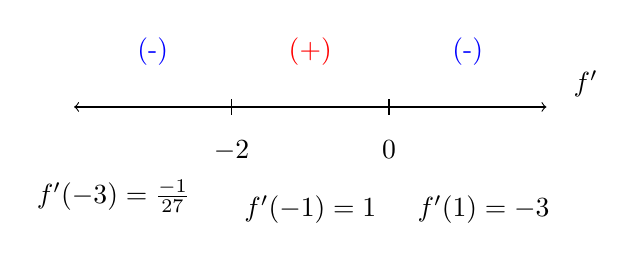
\begin{tikzpicture}
             \draw [<->] (-4,0) -- (2,0);
             \draw (0,0.1) -- (0,-0.1);
             \draw (-2,0.1) -- (-2,-0.1);
             \draw (-2,-0.3)node[below]{$-2$};
             \draw (0,-0.3)node[below]{$0$};
             \draw (-3.5,-0.8)node[below]{$f'(-3) = \frac{-1}{27}$};
             \draw (-1,-1)node[below]{$f'(-1) = 1$};
             \draw (1.2,-1)node[below]{$f'(1) = -3$};
             \draw[red] (-1,1)node[below]{(+)};
             \draw[blue] (1,1)node[below]{(-)};
             \draw[blue] (-3,1)node[below]{(-)};
             \draw (2.5,0)node[above]{$f'$};
           \end{tikzpicture}
         \end{image}
       \end{center}

       So we see that $f$ is increasing on $(-2,0)$, and $f$ is decreasing on $(-\infty, -2)$ and $(0,\infty)$.
       
     \item
       \dfn{Local Extrema}  \\
       $f'$ changes from negative to positive at $x=-2$, so this is the location of a local minimum.
       $f'$ also changes from positive to negative at $x=0$, but $f$ is not defined at $x=0$ and so this is not a local extreme value.
       $f$ has a local minimum at $\left( -2,\frac{3}{4} \right)$.
			
			
			
     \item
       \dfn{Concavity}
       \begin{align*}
         f''(x) &= \frac{x^3(-1) - (-x-2)(3x^2)}{x^6} \\
                &= \frac{-x^3 + 3x^3 + 6x^2}{x^6} \\
		&= \frac{2x^3 + 6x^2}{x^6} \\
		&= \frac{2x+6}{x^4} \\
		&= \frac{2(x+3)}{x^4}
       \end{align*}
			
       To find where $f''$ is positive and where $f''$ is negative, we need to find where $f''(x) = 0$ and where $f''(x)$ does not exist.
       Clearly, $f''(x)$ does not exist when $x=0$.
       To find when $f''(x) = 0$, we solve:
       \begin{align*}
         \frac{2(x+3)}{x^4} = 0 &\implies 2(x+3) = 0\\
         &\implies x=-3
       \end{align*}

	The denominator of $f''$ is always positive so the sign of $f''$ depends on the numerator.  When $x<-3, f''<0$ and when $x>-3, f''>0$.		
									
       To see where $f$ is concave up and concave down, consider the following sign chart for $f''$:
       \begin{center}
         \begin{image}
           \begin{tikzpicture}
             \draw [<->] (-5,0) -- (2,0);
             \draw (0,0.1) -- (0,-0.1);
             \draw (-3,0.1) -- (-3,-0.1);
             \draw (-3,-0.3)node[below]{$-3$};
             \draw (0,-0.3)node[below]{$0$};
             \draw[red] (-1.5,1)node[below]{(+)};
             \draw[red] (1,1)node[below]{(+)};
             \draw[blue] (-4,1)node[below]{(-)};
             \draw (2.5,0)node[above]{$f''$};
           \end{tikzpicture}
         \end{image}
       \end{center}

       So we see that $f$ is concave up on $(-3,0)$ and $(0,\infty)$, and $f$ is concave down on $(-\infty, -3)$.
     \item
       \dfn{Inflection Points}  \\
       $f''(x)$ changes sign from negative to positive at $x=-3$ so $f$ has an inflection point at $\left( -3, \frac{7}{9} \right)$
			
     \item
       \dfn{The graph of $f$}
       \begin{image}
         \includegraphics[scale=.5]{Figure6.png}
       \end{image}

    \end{enumerate}
  \end{freeResponse}
\end{problem}



%probem4
\begin{problem}
  Given that:
  \begin{align*}
    \lim_{x \to - \infty} f(x) &= 0 & \lim_{x \to -3^-} f(x) &= \infty  & \lim_{x \to -3^+} f(x) &= - \infty & \lim_{x \to 4^-} f(x) &= \infty\\
  \lim_{x \to 4^+} f(x) &= -\infty & f(1) &= 1 & f(5) &= -2 && \\
    f'(1) &\ne 0 & f'(7) &= 0 & f'(x) &= 2 \text{ for } x > 9 & f''(1) &= 0 &
 \end{align*}
     the domain of $f$ is: $(-\infty,-3) \cup (-3,4) \cup (4,\infty)$ and $f$ is continuous on its domain.
The following sign chart for the first and second derivatives of $f$:
  \begin{image}
    \includegraphics[scale=.8]{Figure8.png}
  \end{image}
	
find the following:
  \begin{enumerate}
     \item  Critical points.
     \item  Intervals where $f$ is increasing and decreasing.
     \item  Local extrema.
     \item  Inflection points.
     \item  Intervals of concavity.
     \item  Sketch the graph of $f$.
	
  \end{enumerate}
  \begin{freeResponse}
    \begin{enumerate}
      \item
        Critical points. \\
	The critical points of $f$ occur at points in the domain of $f$ where either $f'(x)=0$ or where $f'(x)$ does not exist.  Even though $f'(-3), f'(4),$ and $f'(9)$ do not exist, all three of those points are not in the domain of $f$ and therefore are not critical points.  
        We are given that $f'(7)=0$, and so $x=7$ is a critical point of $f$.
                Therefore, $x=7$ is the only critical point of $f$.  
			
      \item
        Intervals where $f$ is increasing and decreasing.  \\
        $f$ is increasing when $f'(x)>0$.
        From the sign chart and our critical points, these are the intervals $(-\infty ,-3)$, $(-3,4)$, $(4,7]$, and $(9,\infty )$.
        $f(x)$ is decreasing when $f'(x)<0$.
        From the sign chart, this is on the interval $[7,9)$.
			
      \item
        Local extrema.  \\
        Using the first derivative test, $f(7)$ is a local maximum because the derivative changes sign from positive to negative.
        Although the derivative changes sign from negative to positive at $f(9)$, this is not a local minimum because the function is not defined at this point.
        Therefore, $x=7$ is the only local extremum of $f$, and it is a local maximum.
			
      \item
        Inflection points.  \\
        Possible inflection points occur where $f''(x)=0$ or where $f''(x)$ does not exist.
        We are given that $f''(1)=0$.
        In addition, $f''(x)$ does not exist at $x=-3,4,9$.
        However, these are not inflection points because $f$ is not defined at these points.
        Since $f''$ changes sign at $x=1$, this is in fact an inflection point of $f$.
        We are given that $f(1) = 1$, and so the only inflection point of $f$ is the point $(1,1)$.  
			
      \item
        Intervals of concavity.  \\
        $f(x)$ is concave up when $f''(x)>0$.
        From the sign chart, this is on the intervals $(-\infty ,-3)$ and $(1,4)$.
        $f(x)$ is concave down when $f''(x)<0$.
        From the sign chart, this is on the interval $(-3,1)$ and $(4,9)$.
        
			
      \item
        Sketch the graph of $f$.
        \begin{image}
          \includegraphics[scale=.55]{Figure5.png}
	\end{image}
    \end{enumerate}
  \end{freeResponse}
\end{problem}


%problem5
\begin{problem}
  Determine the following information about the given function and then graph the function:
  \[
    f(x) = 3\sin\left(\frac{x}{2}\right), [-2\pi,2\pi]
  \]

 Domain\\
  $x,y$-intercepts\\
  Symmetry\\
  Asympotes\\
  Intervals of increasing/decreasing\\
  Maxima/Minima\\
  Inflection points\\
    Intervals of concavity
    Sketch a graph of $f$

\begin{freeResponse}
\begin{enumerate}

\item Domain: This was given as $[-2\pi,2\pi]$

\item $x,y$-intercepts:\\
x-interpects occur when $f(x) = 3\sin\left(\frac{x}{2}\right)=0 \implies \frac{x}{2}=0+k\pi$ where $k$ is an integer, $-1\le k \le 1$.  On the domain this is $x=-2\pi,0,2\pi$.
y-intercepts: $f(0) = 3\sin\left(\frac{0}{2}\right)=0$  The y-intercept is the point $(0,0)$

\item Symmetry:\\
$f(-x)=3\sin\left(\frac{-x}{2}\right)=-3\sin\left(\frac{x}{2}\right) \ne f(x)$ so $f$ is not even
$-f(x)=-3\sin\left(\frac{x}{2}\right)=f(-x)$ so $f$ is odd

\item Intervals of increasing/decreasing:
            \[
              f'(x) = 3 \cos\left(\frac{x}{2}\right) \cdot \frac{1}{2}
              = \frac{3}{2} \cos\left(\frac{x}{2}\right)
            \]
                  Since $f'$ is defined everywhere on $(-2\pi, 2\pi)$ to find
        the critical points we just solve the equation $f'(x) = 0$
        where $-2\pi < x < 2\pi$:
        \begin{align*}
          f'(x) = 0 &\iff \frac{3}{2} \cos\left(\frac{x}{2}\right) = 0
          \\
           &\iff \cos\left(\frac{x}{2}\right) = 0 \\
          &\iff \mbox{$-2\pi < x < 2\pi$ and $x/2 = \pi/2 + n\pi$
            with $n$ an integer}\\
          &\iff \mbox{$-2\pi < x < 2\pi$ and $x = \pi + n2\pi$
            with $n$ an integer}\\
          &\iff \mbox{$x = -\pi$ and $x = \pi$.}
        \end{align*}
        So the only critical points are $x = -\pi$ and $x = \pi$.\\
        
        If $-2\pi <x< -\pi$, it follows that $-\pi<x/2<-\pi /2$ so $x/2$ lies in the third quadrant and $\cos(x/2)<0$. \\
         If $-\pi <x< \pi$, it follows that $-\pi /2<x/2<\pi /2$ so $x/2$ lies in the fourth and first quadrants and $\cos(x/2)>0$.  \\
         If $\pi <x< 2\pi$, it follows that $\pi /2<x/2<\pi$ so $x/2$ lies in the second quadrant and $\cos(x/2)<0$


         $\implies f$ is increasing on the interval $(-\pi, \pi)$, and $f$ is
        decreasing on the intervals $(-2\pi, -\pi)$ and $(\pi, 2\pi)$.
     
\item Maxima/minima:
 
       Using the sign chart above, the first derivative test states
        we have a local maximum if the sign of $f'$ changes from
        positive to negative, and a local minimum if the sign of $f'$
        changes from negative to positive.

        Therefore there is a local maximum at $x = \pi$ and local
        minimum at $x = -\pi$.
        
        
     \item Intervals of concavity:
      Concavity can change at  interior points in $[-2\pi, 2\pi]$
            where $f''$ is undefined or equal to 0 are only
            \emph{candidates} for the inflection points.  
             \[
          f''(x) = \frac{-3}{2} \sin\left(\frac{x}{2}\right) \cdot
          \frac{1}{2} = \frac{-3}{4} \sin\left(\frac{x}{2}\right)
        \]
$\frac{-3}{4} \sin\left(\frac{x}{2}\right)=0$ when $\sin\left(\frac{x}{2}\right)=0$ which in the domain of $-2\pi < x < 2\pi$ occurs at $x/2 = n\pi$ with $n$ an integer.
$-2\pi < x < 2\pi$ and $x =  n2\pi$   with $n$ an integer $\implies x = 0$

We have a candidate for an inflection point at $x=0$. \\
 If $-2\pi <x< 0$, it follows that $-\pi<x/2<0$ so $x/2$ lies in the third and fourth quadrant and $\sin(x/2)<0$. \\
  If $0 <x<2 \pi$, it follows that $0<x/2<\pi$ so $x/2$ lies in the first and second quadrant and $\sin(x/2)>0$. \\


            So $f$ is concave up on the interval $(-2\pi, 0)$, and $f$
            is concave down on the interval $(0, 2\pi)$.   
    \item Inflection points: 
             Inflection points only occur where the concavity of a
            function changes. Those interior points in $[-2\pi, 2\pi]$
            where $f''$ is undefined or equal to 0 are only
            \emph{candidates} for the inflection points.  We found in part f that we had a candidate for an inflection point at $x=0$.  We verified in part f that concavity changes at $x=0$.
            


            Thus we have that $x = 0$ is the only inflection point.  $f(0)=3\sin\left(\frac{0}{2}\right)=0$.  The inflection point is $(0,0)$
            
            

   

  \item Sketch the graph: 
        \begin{image}
        \includegraphics[scale = .8]{"Graph of function".png}
      \end{image}
  
  
\end{enumerate}
\end{freeResponse}
\end{problem}


%problem6
\begin{problem}
  Determine the following information about the given function and then graph the function:
  \[
    f(x) = x\ln(x)
  \]

 Domain\\
  $x,y$-intercepts\\
  Symmetry\\
  Intervals of increasing/decreasing\\
  Maxima/Minima (including absolute)\\
  Intervals of concavity\\
  Inflection points
Given $\lim{x \to 0^+}=0$, sketch a graph $f$.

\begin{freeResponse}
\begin{enumerate}


\item Domain: $(0,\infty)$

\item $x,y$-intercepts:\\
x-interpects occur when $f(x) = x\ln(x) =0$.  We would think this occurs when either $x=0$ or $ln(x)=0$.  However, $x=0$ is not in the domain.  We only have $ln(x)=0$ which is at $x=1$.
y-intercepts: None given the domain.


\item Symmetry: Given the domain of the function, it does not make sense to check for even/odd.

\item Intervals of increasing/decreasing:

$$f'(x)=\ln(x)+1$$
Find: $f'(x)=\ln(x)+1=0 \implies \ln(x)=-1 \implies x=e^{-1}$\\

Since $f'$ possibly changes its sign at critical points only, the sign of $f'$ is constant on intervals $(0,e^{-1})$ and $(e^{-1},\infty)$. 
Since $f'(1)=1>0$, and $f'(e^{-3})=-3+1=-2<0$, it follows that $f'$ is negative on $(0,e^{-1})$ and positive on $(e^{-1},\infty)$. 

Therefore, $f$ is decreasing on $(0,e^{-1})$ and $f$ is increasing on $(e^{-1},\infty)$. 

\item  Maxima/Minima

Since the function is decreasing on $(0,e^{-1})$ and $f$ is increasing on $(e^{-1},\infty)$., the absolute minimum value of $f$ is attained at $x=e^{-1}$.  The absolute minimum value of $f(x)=f(e^{-1})=e^{-1}\ln e^{-1}=-e^{-1}=-\frac{1}{e}$

The absolute maximum value of $f$ does not exist, since the only critical point is a minimum and $\lim{x \to \infty}f(x)=+\infty$

\item Intervals of concavity and inflection points:
$f'(x)=\ln(x)+1 \implies f''(x)=\frac{1}{x}>0$ on the domain of $f$.  Concave up on its domain and there are no inflection points.

\item Given $\lim{x \to 0^+}=0$, sketch a graph $f$:
        \begin{image}
        \includegraphics[scale = .7]{figure7.png}
      \end{image}





\end{enumerate}
\end{freeResponse}
\end{problem}


%problem7
\begin{problem}
  Sketch a graph of the function $f$ defined by
  \[
    f(x) = \begin{cases}
             2x - 2\tan^{-1}(x) - x \ln(x^2+1) & \mbox{for $x \le 1$}\\
             \sqrt{x - 2} & \mbox{for $x \ge 2$}
           \end{cases}
  \]
  \begin{enumerate}
    \item Find the domain of $f$.
      \begin{freeResponse}
        The domain of $f$ is $(-\infty, 1] \cup [2, \infty)$.
      \end{freeResponse}

    \item Show that $f'(x) = -\ln(x^2+1)$ on the interval $(-\infty, 1)$.
   \begin{freeResponse}
        For $x < 1$ we have
        \begin{align*}
          f'(x) &= 2 - \frac{2}{1+x^2} - \ln(x^2+1) - x \cdot \frac{1}{x^2+1}\cdot 2x\\
                &= 2 - \frac{2}{1+x^2} - \ln(x^2+1) - \frac{2x^2}{x^2+1}\\
                &= 2 - \frac{2 + 2x^2}{x^2+1} - \ln(x^2+1)\\
                &= 2 -  2\cdot\frac{1+x^2}{x^2+1} - \ln(x^2+1)\\
                &= 2 - 2 - \ln(x^2 +1) = -\ln(x^2+1)
        \end{align*}
      \end{freeResponse}

    \item Compute a formula for $f'$ on the interval $(2, \infty)$.
      \begin{freeResponse}
        For $x > 2$ we have
        \begin{align*}
          f'(x) &= \frac{1}{2\sqrt{x-2}}
        \end{align*}
      \end{freeResponse}

    \item Compute a formula for $f''$ on the interval $(-\infty, 1)$.
       \begin{freeResponse}
        For $x < 1$ we have
        \begin{align*}
          f''(x) &= \frac{-1}{x^2+1} \cdot 2x = \frac{-2x}{x^2+1}
        \end{align*}
      \end{freeResponse}

    \item Compute a formula for $f''$ on the interval $(2, \infty)$.
 \begin{freeResponse}
        For $x>2$ we have
        \begin{align*}
          f''(x) &= \frac{-1}{4(x-2)^{-3/2}}
        \end{align*}
      \end{freeResponse}


    \item List all the asymptotes (with limit justifications, if appropriate).
      (If $f$ does not have a particular asymptote write ``NONE''.)
      \begin{enumerate}
        \item
          Vertical asymptotes:
              \begin{freeResponse}
            NONE: For $x \ge 2$, $f(x)=\sqrt{x - 2}$ so no vertical asymptotes there.  For $x \le 1,\ f(x)= 2x - 2\tan^{-1}(x) - x \ln(x^2+1)$ we can look at each term.  The term $2x$ is a polynomial.  The term $- 2\tan^{-1}(x)$ is bounded.  Finally, the term $- x \ln(x^2+1)$.  We would be concerned about where $x^2+1=0$ but that never happens because of the squared term.
          \end{freeResponse}

        \item
          Horizontal asymptotes:
           \begin{freeResponse}
            No H.A. as $x \to \infty$:
            \begin{align*}
              \lim_{x\to\infty} f(x) &= \lim_{x \to \infty} \underbrace{\sqrt{x-2}}_{\text{form $\infty$}} = \infty
            \end{align*}

            No H.A. as $x \to -\infty$:
            \begin{align*}
              \lim_{x \to -\infty} f(x) &= \lim_{x \to -\infty} 2x - 2\tan^{-1}(x) - x \ln(x^2+1)\\
              &= \lim_{x \to -\infty} \left[x\cdot(2 - \ln(x^2+1)) - 2\tan^{-1}(x)\right]\\
              &= \lim_{x \to -\infty} \left[x \cdot(2 + \ln(x^2+1)^{-1} -2\tan^{-1}(x) \right]\\
              &= \lim_{x \to -\infty} \left[\underbrace{x}_{\text{$\to -\infty$}} \cdot \left(2 + \ln\left(\underbrace{\frac{1}{x^2+1}}_{\text{$\to 0$}}\right)\right) -2\underbrace{\tan^{-1}(x)}_{\text{$\to -\pi/2$}} \right]\\
              &= \lim_{x \to -\infty} \left[\underbrace{x}_{\text{$\to -\infty$}} \cdot \left( 2 + \underbrace{2 + \ln(1/(x^2+1))}_{\to -\infty}\right) -\underbrace{2\tan^{-1}(x)}_{\text{$\to -\pi$}} \right]\\
              &= \infty
            \end{align*}
          \end{freeResponse}
      \end{enumerate}

    \item
      In the following sign chart for $f'$, list the points (in the domain of $f$) where $f'(x) = 0$ or $f'(x)$ is undefined, indicate the sign of $f'$ on each subinterval, and identify any local extrema (with ``local max'' or ``local min''.)
      In the following sign chart for $f''$, list the points (in the domain of $f$) where $f''(x) = 0$ or $f''(x)$ is undefined, indicate the sign of $f''$ on each subinterval, and identify any inflection points.
      Use this information to sketch a graph of $f$ in the blank grid.
      (Be sure to indicate any $x$- or $y$-intercepts.)
        \begin{image}
          \includegraphics[scale = 0.2]{"Blank grid with number lines".png}
        \end{image}
        
           \begin{freeResponse}
        \textbf{Finding critical points of $f'$:}

        For $x < 1$ we have
        \begin{align*}
          f'(x) = 0 &\iff -\ln(x^2+1) = 0 \\
          &\iff \ln(x^2+1) = 0\\
          &\iff x^2 + 1 = e^0 = 1\\
          &\iff x = 0.
        \end{align*}
        Critical point at $0$ when $x < 1$.

        For $x > 2$ we have
        \begin{align*}
          f'(x) = 0 &\iff \frac{1}{2\sqrt{x-2}} = 0
        \end{align*}
        This last equation is never true.
        Hence no critical points when $x > 2$.

        Sign chart of $f'$:
        \begin{image}
          \includegraphics[scale = 0.2]{"Sign chart of derivative2".png}
        \end{image}
        
        local max: none
        
        local min: none

        intervals where $f$ is increasing: $(2, \infty)$

        intervals where $f$ is decreasing: $(-\infty, 0)$, $(0, 1)$, 

        \textbf{Find candidates for inflection points:}

        For $x < 1$ we have
        \begin{align*}
          f''(x) = 0 &\iff \frac{-2x}{x^2+1} = 0\\
          &\iff x = 0.
        \end{align*}
        So, $x=0$ is a candidate for an inflection point. 

        For $x > 2$ we have
        \begin{align*}
          f''(x) = 0 &\iff \frac{-1}{4(x-2)^{3/2}} = 0
        \end{align*}
        This last equation has no solution.
        Hence no candidates for inflection points when $x >2$.

        We need to determine the sign of $f''$ on the intervals $(-\infty,0), (0,1), (2,\infty)$.
        \begin{image}
          \includegraphics[scale = 0.3]{figure11.png}
        \end{image}
        
        

       $f''$ changes sign at $x=0$ so $(0,0)$ is an inflection point.

        intervals where $f$ is concave up: $(-\infty, 0)$

        intervals where $f$ is concave down: $(0,1)$, $(2, \infty)$

        Final sketch of graph:
        \begin{image}
          \includegraphics[scale = 0.4]{"Final graph".png}
        \end{image}
      \end{freeResponse}
        
        
    \end{enumerate}
\end{problem}


\end{document} 
